\RequirePackage{plautopatch}
\RequirePackage[l2tabu, orthodox]{nag}

\documentclass[
  platex,           % 使用するコンパイラ(2023年2月時点のCloud LaTeXではplatexがデフォルトで使用されている)
  dvipdfmx,         % ドライバ
  fontsize=10pt,    % 欧文フォントサイズの指定
  jafontsize=10pt,  % 和文フォントサイズの指定
  book,             % bookクラスを選択
  openany,          % 章が変わったときの空白ページ自動挿入をしない
]{jlreq}

\usepackage[
  top=20truemm,
  bottom=20truemm,
  left=20truemm,
  right=20truemm]{geometry}         % 余白設定
\usepackage{graphicx}               % 図や画像などのグラフィックを扱う
\usepackage{svg}                   % svg画像を扱う
\usepackage{booktabs}               % 論文に使用されるような表を出力
\usepackage{amsmath, amssymb}       % 数式表現パッケージ
\usepackage[
  dvipdfmx,
  bookmarksnumbered=true]{hyperref} % しおりを作成
\usepackage{pxjahyper}              % 日本語のしおりを作成
\usepackage{subfigure}              % サブフィギュア

\begin{document}
\pagenumbering{alph}
\thispagestyle{empty}
\begin{center}
  \vspace*{20mm}
  {\LARGE 学 士 学 位 論 文\\}
  \vfill
  \textbf{{\huge AutoEncoderを用いた特徴量拡張による\\教師あり学習の精度向上に関する研究\\}}
  \vfill
  {\LARGE 令和5年度\\}
  \vfill
  {\LARGE 茨城大学工学部\\}
  \vfill
  {\LARGE 機械システム工学専攻\\}
  {\LARGE 佐藤 竜太\\}
  \vspace*{20mm}
\end{center}
\newpage
  % タイトル情報
\pagenumbering{roman}             % ページ番号をローマ数字で記載
% 日本語-------------------------
\phantomsection % 目次のリンクのために使用
\addcontentsline{toc}{chapter}{要旨} % 目次に要旨を追加
\begin{center}
  \textbf{{\LARGE AutoEncoderを用いた特徴量拡張による教師あり学習の精度向上に関する研究\\}}
  \vspace{5mm}
  {\large 茨城大学 工学部 機械システム工学科\\
  佐藤 竜太\\}
  \vspace{5mm}
  {\large 要旨}
  \vspace{5mm}
\end{center}
ここに本文.ここに本文.ここに本文.ここに本文.ここに本文.ここに本文.

\newpage

% 英語-------------------------
\begin{center}
  \textbf{{\LARGE Title Here\\}}
  \vspace{5mm}
  {\large Major in Mechanical Systems Engineering,\\ Ibaraki University\\
  Kanta SHIBATA\\}
  \vspace{5mm}
  {\large Abstract}
  \vspace{5mm}
\end{center}
Here is text. Here is text. Here is text. Here is text. Here is text.
    % 概要(日本語,英語)
\tableofcontents                  % 目次
\newpage
\listoffigures                    % 図目次
\newpage
\listoftables                     % 表目次
\newpage

\pagenumbering{arabic}            % ページ番号をアラビア数字
\chapter{序論}
\section{背景}
ここに文.ここに文.ここに文.ここに文.ここに文.ここに文.ここに文.ここに文.ここに文.ここに文.ここに文.ここに文.ここに文.ここに文.ここに文.ここに文.ここに文.ここに文.ここに文.ここに文.ここに文.ここに文.ここに文.ここに文.ここに文.ここに文.ここに文.ここに文.
\subsection{背景1}
ここに文.ここに文.ここに文.ここに文.ここに文.ここに文.ここに文.ここに文.ここに文.ここに文.ここに文.ここに文.ここに文.ここに文.ここに文.ここに文.ここに文.ここに文.ここに文.ここに文.ここに文.ここに文.ここに文.ここに文.ここに文.ここに文.ここに文.ここに文.
\subsection{背景2}
ここに文.ここに文.ここに文.ここに文.ここに文.ここに文.ここに文.ここに文.ここに文.ここに文.ここに文.ここに文.ここに文.ここに文.ここに文.ここに文.ここに文.ここに文.ここに文.ここに文.ここに文.ここに文.ここに文.ここに文.ここに文.ここに文.ここに文.ここに文.
\section{目的}
ここに文.ここに文.ここに文.ここに文.ここに文.ここに文.ここに文.ここに文.ここに文.ここに文.ここに文.ここに文.ここに文.ここに文.ここに文.ここに文.ここに文.ここに文.ここに文.ここに文.ここに文.ここに文.ここに文.ここに文.ここに文.ここに文.ここに文.ここに文.
\section{構成}
ここに文.ここに文.ここに文.ここに文.ここに文.ここに文.ここに文.ここに文.ここに文.ここに文.ここに文.ここに文.ここに文.ここに文.ここに文.ここに文.ここに文.ここに文.ここに文.ここに文.ここに文.ここに文.ここに文.ここに文.ここに文.ここに文.ここに文.ここに文.

\chapter{図表を載せる}
図\ref{fig:sin}のように参照できる.
同様に表\ref{tab:demo}のように参照できる.

\begin{figure}[h]
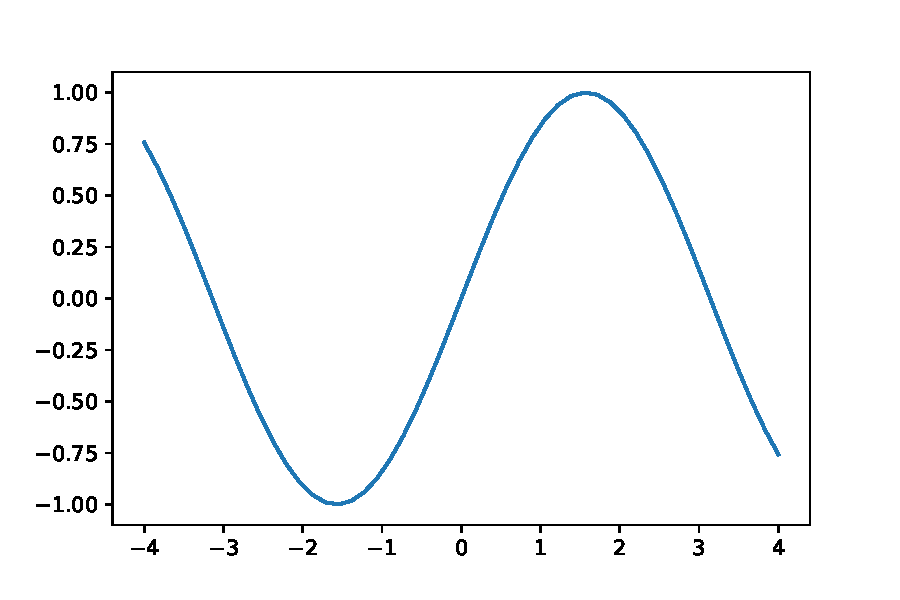
\includegraphics[scale=0.8]{figures/sample-figure.pdf}
\centering
\caption{正弦波}
\label{fig:sin}
\end{figure}

\begin{table}[h]
\centering
\caption{サンプル}
\label{tab:demo}
\begin{tabular}{@{}llr@{}}
\toprule
\multicolumn{2}{c}{Item} &            \\ \cmidrule(r){1-2}
Animal     & Description & Price (\$) \\ \midrule
Gnat       & per gram    & 13.65      \\
           & each        & 0.01       \\
Gnu        & stuffed     & 92.50      \\
Emu        & stuffed     & 33.33      \\
Armadillo  & frozen      & 8.99       \\ \bottomrule
\end{tabular}
\end{table}


\newpage
\phantomsection
\addcontentsline{toc}{chapter}{謝辞}
\section*{謝辞}
研究を進めるにあたり,研究の方向性や,理解の行き届いていない点について手厚くご指導いただいた近藤久先生に厚く御礼申し上げます.また,研究に関する多くの助言をいただいた近藤研究室の皆様に感謝いたします.おかげさまで,機械学習分野への知識の幅を広げることができました. % 謝辞

\newpage
\phantomsection
\addcontentsline{toc}{chapter}{参考文献}  % 目次に参考文献を追加
\bibliographystyle{junsrt}                % 参考文献のスタイル
\bibliography{contents/references.bib}    % 参考文献を表示
\end{document}
